
\section{Metodolog�a HAR}
\begin{frame}{Metodolog�a HAR}

\framesubtitle{Proceso de aprendizaje}
\begin{center}
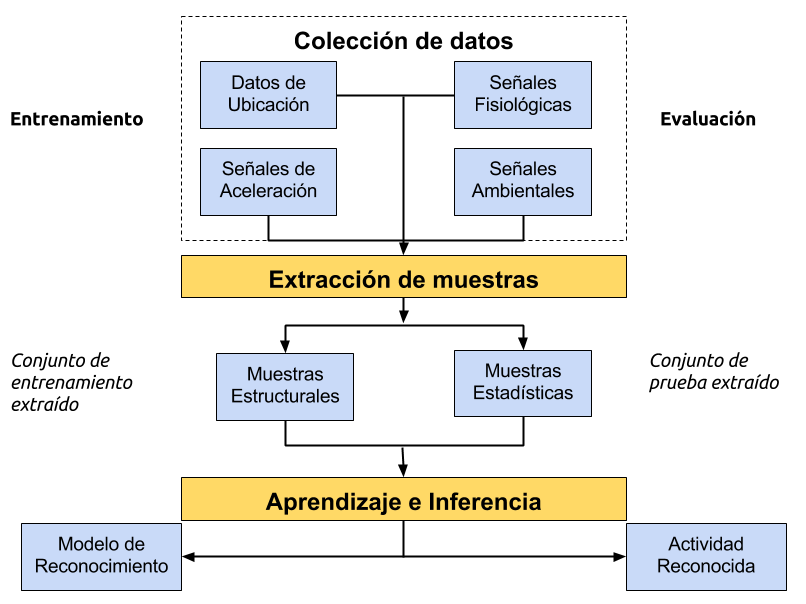
\includegraphics[width=8cm]{../capitulo-2/graphics/harsystem}
\par\end{center}

\end{frame}
%
\begin{frame}{Metodolog�a HAR}
\framesubtitle{Proceso de aprendizaje}
\begin{itemize}
	\item Como en otros m�todos de aprendizaje autom�tico, el proceso de reconocimiento se divide en dos etapas conocidas:
	\begin{itemize}
		\item Entrenamiento
		\item Evaluaci�n
	\end{itemize}
	\item En el entrenamiento requiere:
		\begin{itemize}
			\item Colecta de conjunto de Datos en series de tiempo.
			\item Se realiza la extracci�n de muestras en ventanas de tiempo, calculando las caracter�sticas de entrenamiento.
			\item Se genera un modelo de Reconocimiento de Actividades a trav�s de un m�todo de aprendizaje autom�tico.
		\end{itemize}
	\item En la evaluaci�n, de igual manera, se recopila los datos, se realiza la extracci�n de muestras y calculo de las mismas caracter�sticas del entrenamiento, de modo a evaluar el modelo generado.
\end{itemize}
\end{frame}
%
\begin{frame}{Metodolog�a HAR}
\framesubtitle{Colecci�n de Datos}
	\begin{itemize}
		\item El primer paso es recolectar se�ales obtenidas de sensores unidos al cuerpo (cintura, mu�eca, muslos, etc).
		
		\item El m�todo de grabaci�n consiste en capturar las se�ales de un sensor o m�s sensores a un individuo realizando alguna actividad de inter�s.
		
		\item Las se�ales de sensores pueden clasificarse seg�n el movimiento, la posici�n, el entorno y la fisiolog�a.	
	\end{itemize}
\end{frame}
%
\begin{frame}{Metodolog�a HAR}
\framesubtitle{Colecci�n de Datos}
\begin{center}
\resizebox{\linewidth}{!}{
\begin{tabular}{|c|c|c|c|c|c|c|c|}
	\hline 
	\multicolumn{8}{|c|}{Sensores} \\ 
	\hline 
	\multicolumn{2}{|c|}{Movimiento}	& \multicolumn{2}{c|}{Posici�n} 	& \multicolumn{2}{c|}{Ambientales}  	& \multicolumn{2}{c|}{Fisiol�gicas}  		\\ 
	\hline 
	
\includegraphics[width=0.05\textwidth]{propuesta/graphics/acelerometro} 	& Acelerometro 		&
	
\includegraphics[width=0.04\textwidth]{propuesta/graphics/barometro}		& Bar�metro			&
	
\includegraphics[width=0.05\textwidth]{propuesta/graphics/camera}			& Camara			&
	
\includegraphics[width=0.05\textwidth]{propuesta/graphics/ritmo_cardiaco}	& Ritmo Card�aco	
	\\
	
\includegraphics[width=0.05\textwidth]{propuesta/graphics/giroscopio} 		& Giroscopio 		&
	
\includegraphics[width=0.05\textwidth]{propuesta/graphics/gps}				& GPS				&
	
\includegraphics[width=0.05\textwidth]{propuesta/graphics/microfono}		& Micr�fono			&
	
\includegraphics[width=0.05\textwidth]{propuesta/graphics/temperatura}		& Temperatura		
	\\
	
\includegraphics[width=0.05\textwidth]{propuesta/graphics/magnetometro} 	& Magnet�metro		&
	
\includegraphics[width=0.05\textwidth]{propuesta/graphics/wifi}				& WIFI				&
	
\includegraphics[width=0.05\textwidth]{propuesta/graphics/luz}				& Luz				&
																				&  						
	\\
	
\includegraphics[width=0.05\textwidth]{propuesta/graphics/pedometro}		& Pod�metro			&	
	
\includegraphics[width=0.05\textwidth]{propuesta/graphics/gsm}				& GSM				&
	
\includegraphics[width=0.05\textwidth]{propuesta/graphics/proximidad}		& Proximidad		&	
																				&					
	\\
	\hline 
\end{tabular}
} % fin del resize
\end{center}
\end{frame}
%
\begin{frame}{Metodolog�a HAR}
\framesubtitle{Extracci�n de Muestras}
	
\end{frame}
%
\begin{frame}{Metodolog�a HAR}	
\framesubtitle{Aprendizaje}
	
\end{frame}
%


%	\begin{figure}[ht]
%		\includemovie[
%		poster,
%		text={\small(Loading activitySurvey.mp4)}
%		]{6cm}{6cm}{propuesta/activitySurvey.mp4}
%	\end{figure}